% One-page architecture of the Round 3 agents (shop moss-and-oak, buyer move_76).
% Build: pdflatex architecture.tex
\documentclass[border=8pt]{standalone}
\usepackage[T1]{fontenc}
\usepackage{lmodern}
\usepackage{tikz}
\usetikzlibrary{positioning,fit,arrows.meta,backgrounds,calc}

\definecolor{code}{HTML}{2F6B9A}
\definecolor{model}{HTML}{B5532A}
\definecolor{mem}{HTML}{3C7D4A}
\definecolor{tool}{HTML}{6B5B95}
\definecolor{mkt}{HTML}{555555}

\tikzset{
  box/.style={draw, rounded corners=2pt, align=left, font=\footnotesize, inner sep=4pt, text width=#1},
  box/.default=4.6cm,
  codebox/.style={box=#1, draw=code, fill=code!7},
  modelbox/.style={box=#1, draw=model, fill=model!9},
  membox/.style={box=#1, draw=mem, fill=mem!8},
  toolbox/.style={box=#1, draw=tool, fill=tool!8},
  mktbox/.style={box=#1, draw=mkt, fill=mkt!6},
  lane/.style={draw=#1!60, dashed, rounded corners=4pt, inner sep=6pt},
  title/.style={font=\small\bfseries, anchor=north west},
  arr/.style={-{Stealth[length=2mm]}, thick, #1},
  arr/.default=black!70,
  lbl/.style={font=\scriptsize, fill=white, inner sep=1pt, align=center},
}

\begin{document}
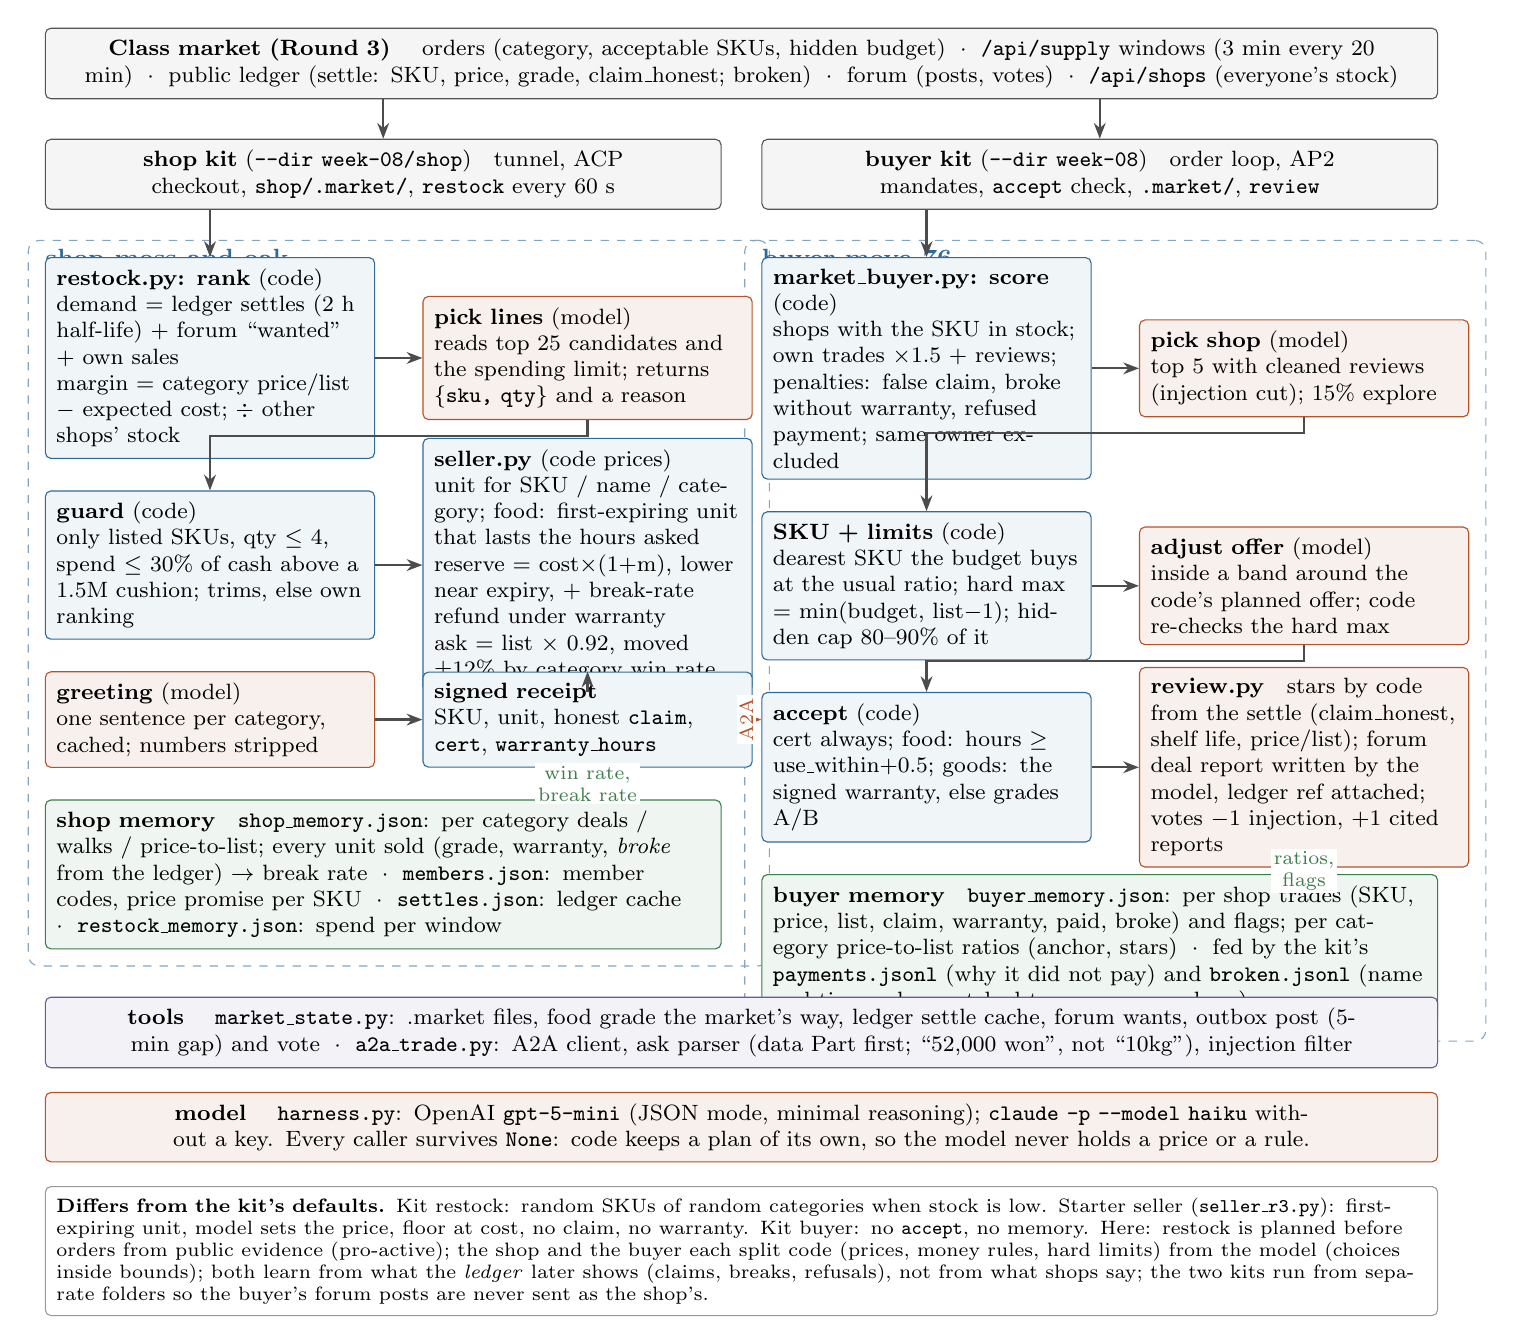
\begin{tikzpicture}[node distance=4mm and 6mm]

% ---------------- market
\node[mktbox=17.4cm, align=center] (market) {\textbf{Class market (Round 3)} \quad
  orders (category, acceptable SKUs, hidden budget) \;$\cdot$\; \texttt{/api/supply} windows (3 min every 20 min) \;$\cdot$\;
  public ledger (settle: SKU, price, grade, claim\_honest; broken) \;$\cdot$\; forum (posts, votes) \;$\cdot$\; \texttt{/api/shops} (everyone's stock)};

% ---------------- kits
\node[mktbox=8.3cm, below=5mm of market.south west, anchor=north west, align=center] (skit)
  {\textbf{shop kit} (\texttt{--dir week-08/shop}) \; tunnel, ACP checkout, \texttt{shop/.market/}, \texttt{restock} every 60 s};
\node[mktbox=8.3cm, below=5mm of market.south east, anchor=north east, align=center] (bkit)
  {\textbf{buyer kit} (\texttt{--dir week-08}) \; order loop, AP2 mandates, \texttt{accept} check, \texttt{.market/}, \texttt{review}};

% ---------------- shop lane
\node[codebox=3.9cm, below=6mm of skit.south west, anchor=north west] (rank)
  {\textbf{restock.py: rank} (code)\\ demand = ledger settles (2 h half-life) + forum ``wanted'' + own sales\\
   margin = category price/list $-$ expected cost; $\div$ other shops' stock};
\node[modelbox=3.9cm, right=of rank] (rpick)
  {\textbf{pick lines} (model)\\ reads top 25 candidates and the spending limit; returns \texttt{\{sku, qty\}} and a reason};
\node[codebox=3.9cm, below=of rank] (rguard)
  {\textbf{guard} (code)\\ only listed SKUs, qty $\le$ 4, spend $\le$ 30\% of cash above a 1.5M cushion; trims, else own ranking};
\node[codebox=3.9cm, right=of rguard] (sell)
  {\textbf{seller.py} (code prices)\\ unit for SKU / name / category; food: first-expiring unit that lasts the hours asked\\
   reserve = cost$\times$(1+m), lower near expiry, $+$ break-rate refund under warranty\\
   ask = list $\times$ 0.92, moved $\pm$12\% by category win rate};
\node[modelbox=3.9cm, below=of rguard] (greet)
  {\textbf{greeting} (model)\\ one sentence per category, cached; numbers stripped};
\node[codebox=3.9cm, right=of greet] (rcpt)
  {\textbf{signed receipt}\\ SKU, unit, honest \texttt{claim}, \texttt{cert}, \texttt{warranty\_hours}};
\node[membox=8.3cm, below=of greet.south west, anchor=north west] (smem)
  {\textbf{shop memory} \; \texttt{shop\_memory.json}: per category deals / walks / price-to-list; every unit sold
   (grade, warranty, \textit{broke} from the ledger) $\rightarrow$ break rate \;$\cdot$\; \texttt{members.json}: member codes,
   price promise per SKU \;$\cdot$\; \texttt{settles.json}: ledger cache \;$\cdot$\; \texttt{restock\_memory.json}: spend per window};

% ---------------- buyer lane
\node[codebox=3.9cm, below=6mm of bkit.south west, anchor=north west] (score)
  {\textbf{market\_buyer.py: score} (code)\\ shops with the SKU in stock; own trades $\times$1.5 + reviews;
   penalties: false claim, broke without warranty, refused payment; same owner excluded};
\node[modelbox=3.9cm, right=of score] (bpick)
  {\textbf{pick shop} (model)\\ top 5 with cleaned reviews (injection cut); 15\% explore};
\node[codebox=3.9cm, below=of score] (sku)
  {\textbf{SKU + limits} (code)\\ dearest SKU the budget buys at the usual ratio; hard max = min(budget, list$-$1);
   hidden cap 80--90\% of it};
\node[modelbox=3.9cm, right=of sku] (band)
  {\textbf{adjust offer} (model)\\ inside a band around the code's planned offer; code re-checks the hard max};
\node[codebox=3.9cm, below=of sku] (acc)
  {\textbf{accept} (code)\\ cert always; food: hours $\ge$ use\_within$+$0.5; goods: the signed warranty, else grades A/B};
\node[modelbox=3.9cm, right=of acc] (post)
  {\textbf{review.py} \; stars by code from the settle (claim\_honest, shelf life, price/list);
   forum deal report written by the model, ledger ref attached; votes $-$1 injection, $+$1 cited reports};
\node[membox=8.3cm, below=of acc.south west, anchor=north west] (bmem)
  {\textbf{buyer memory} \; \texttt{buyer\_memory.json}: per shop trades (SKU, price, list, claim, warranty, paid, broke) and
   flags; per category price-to-list ratios (anchor, stars) \;$\cdot$\; fed by the kit's \texttt{payments.jsonl} (why it did
   not pay) and \texttt{broken.jsonl} (name and time only: matched to our own purchase)};

% ---------------- shared tools and model
\node[toolbox=17.4cm, below=6mm of smem.south west, anchor=north west, align=center] (tools)
  {\textbf{tools} \quad \texttt{market\_state.py}: .market files, food grade the market's way, ledger settle cache,
   forum wants, outbox post (5-min gap) and vote \;$\cdot$\;
   \texttt{a2a\_trade.py}: A2A client, ask parser (data Part first; ``52,000 won'', not ``10kg''), injection filter};
\node[modelbox=17.4cm, below=3mm of tools, align=center] (llm)
  {\textbf{model} \quad \texttt{harness.py}: OpenAI \texttt{gpt-5-mini} (JSON mode, minimal reasoning); \texttt{claude -p --model haiku}
   without a key. Every caller survives \texttt{None}: code keeps a plan of its own, so the model never holds a price or a rule.};

% ---------------- lanes
\begin{scope}[on background layer]
  \node[lane=code, fit=(rank)(rpick)(smem), label={[title, code]north west:\;shop moss-and-oak}] (slane) {};
  \node[lane=code, fit=(score)(bpick)(bmem), label={[title, code]north west:\;buyer move\_76}] (blane) {};
\end{scope}

% ---------------- arrows
\draw[arr] (market.south -| skit.north) -- (skit.north);
\draw[arr] (market.south -| bkit.north) -- (bkit.north);
\draw[arr] (skit.south -| rank.north) -- (rank.north);
\draw[arr] (bkit.south -| score.north) -- (score.north);
\draw[arr] (rank) -- (rpick);
\draw[arr] (rpick.south) -- ++(0,-2mm) -| (rguard.north);
\draw[arr] (rguard) -- (sell);
\draw[arr] (sell) -- (rcpt);
\draw[arr] (greet) -- (rcpt);
\draw[arr] (score) -- (bpick);
\draw[arr] (bpick.south) -- ++(0,-2mm) -| (sku.north);
\draw[arr] (sku) -- (band);
\draw[arr] (band.south) -- ++(0,-2mm) -| (acc.north);
\draw[arr] (acc) -- (post);
\draw[arr=mem] (smem.north -| sell.south) -- node[lbl]{win rate,\\break rate} (rcpt.south);
\draw[arr=mem] (bmem.north -| post.south) -- node[lbl]{ratios,\\flags} (post.south);
\draw[arr=model, dashed] (rcpt.east) -- node[lbl, above, rotate=90]{A2A} (rcpt.east -| score.west);

% ---------------- what differs from the kit's defaults
\node[box=17.4cm, draw=black!40, below=3mm of llm, font=\scriptsize] (diff)
  {\textbf{Differs from the kit's defaults.} Kit restock: random SKUs of random categories when stock is low.
   Starter seller (\texttt{seller\_r3.py}): first-expiring unit, model sets the price, floor at cost, no claim, no warranty.
   Kit buyer: no \texttt{accept}, no memory. Here: restock is planned before orders from public evidence (pro-active);
   the shop and the buyer each split code (prices, money rules, hard limits) from the model (choices inside bounds);
   both learn from what the \emph{ledger} later shows (claims, breaks, refusals), not from what shops say; the two kits
   run from separate folders so the buyer's forum posts are never sent as the shop's.};

\end{tikzpicture}
\end{document}
